% !TEX TS-program = latex
% !TEX root = Thesis_Guo2013.tex

\chapter{Diverging Moments and Their Asymptotics}
In the previous chapter, we have revisited some of the basic concepts in probability and outlined the definition for sample and population moments, along with some of their mathematical properties. In this chapter, we will first clarify the relation between the sample and population moments under convergence and use it as an intuition towards the central topic in this thesis, i.e. the analysis of diverging moments. Then, in the scenario of diverging population moments, we will analyze the behavior of sample moments with the growth of population size. Next, the equiprobable-slice method will be proposed, which is to serve as the key to the asymptotic analysis of diverging moments. When moments converge, the method will be shown to be consistent with the true value of moments; when moments diverge, we will see how to the method to reproduce the asymptotics of divergence.

\section{The relation between sample and population moment under convergence}
For the sake of simplicity, we restrict the moments discussed here to \textit{raw moments}, i.e. moments taken about $ c=0 $. The conclusions can also be applied to moments taken about any other value. Let us consider a random variable $ X $ and assume that its $ k $-th population raw moment $ \mu_k' $  is convergent. Supposing the population distribution is characterized by a PDF $ f(x) $, then $ \mu_k' = \int_{-\infty}^{+\infty} x^kf(x)dx $.

Now supposing we have $ N $ independent and identical distributed (i.i.d.) samples $ X_1, X_2, \cdots, X_N $, we can compute the corresponding sample raw moment as $ m_k' = \frac{1}{N} \sum_{i=1}^N X_i^k $. The distribution of each sample is obviously identical to the population distribution, therefore we have 
\begin{equation*}
\E[m_k'] = \frac{1}{N} \sum_{i=1}^N \E[X_i^k] = \frac{1}{N} \sum_{i=1}^N \int_{-\infty}^{+\infty} x_i^k f(x) dx = \mu_k',
\end{equation*}
which can be equally stated as the theorem below.

\begin{thm}
The sample moment $ m_k' $ is an unbiased estimator for the corresponding population moment $ \mu_k' $, given that $ \mu_k' $ exists (is convergent).
\end{thm}

As sample moments are computed from samples, they are random variables by themselves. Then how can one make the estimation for population moment as precise as possible? It is straightforward to imagine that a sample moment  coming from samples of a large size would be a better estimation than one from a small size. Hence, when the sample size $ N \rightarrow \infty $, can we guarantee that the sample moment equates with population moment? The answer is $ yes $ due to the \textit{Law of Large Numbers}.

\begin{thm}
(The Weak Law of Large Numbers) Let $ X_1, X_2, \cdots, X_N $ be a sequence of independent and identically distributed random variables, each having the same expectation $ \E[X_i]=\mu $ \footnote{An assumption of finite variance $\sigma(X_1)^2 = \sigma(X_2)^2 = \cdots = \sigma^2 < \infty $ is not necessary. Large or infinite variance will make the convergence slower, but the law holds anyway. This assumption is often used because it makes the proofs easier.}
, then their arithmetic mean $ \overline{X}_N = \frac{1}{N} \sum_{i=1}^{N} X_i$ converges in probability towards $ \mu $, i.e. $\lim_{N \rightarrow \infty} P(|\overline{X}_N - \mu|>\epsilon) = 0$ for any positive $ \epsilon $. 
\end{thm}

By the two theorems above, we arrive at the following lemma, which formally states the simple relation between the sample and population moment under convergence. 
\begin{lemma}
A sample moment $ m_k' $ converges in probability towards the corresponding population moment $ \mu_k' $ when the sample size $ N \rightarrow \infty $, given that $ \mu_k' $ exists (is convergent).
\end{lemma}

Fig. \ref{fig:ch2_u4converge} is an example that illustrates how this convergence is realized when the sample size grows bigger. We draw i.i.d. samples from a standard Gaussian distribution and compare the sample $ \mu_4 $ with its population counterpart $ \mu_4=3 $. The convergence is guaranteed when the sample size extends to infinity, as indicated by the trend shown here. 

\begin{figure}[htbp]
\begin{center}
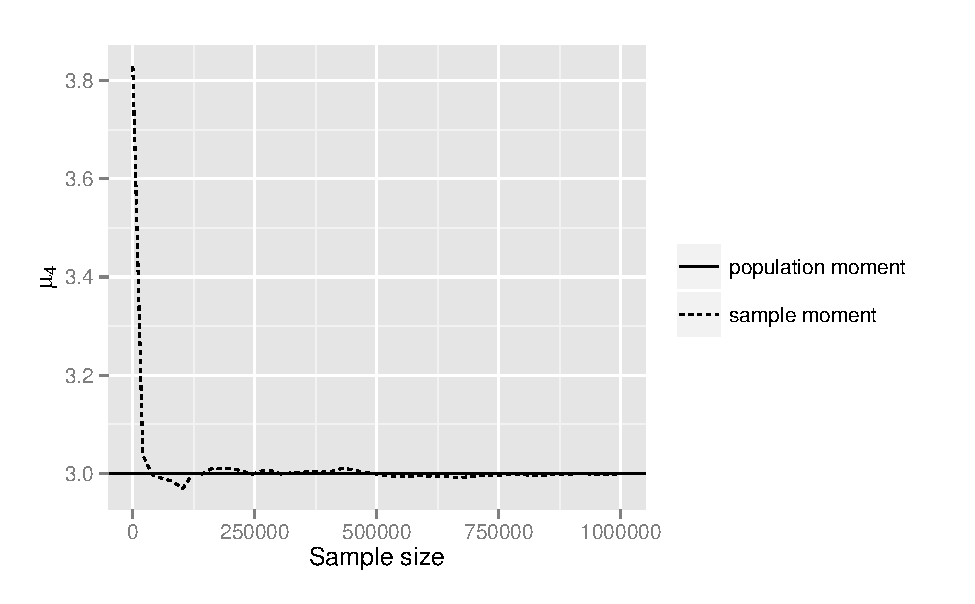
\includegraphics[width=0.9\textwidth]{figures/ch2_u4converge_gauss.eps}
\caption{Moment $ \mu_4 $ computed from i.i.d. samples of growing sample sizes drawn from a standard Gaussian distribution. It can be seen that the sample  moment converges to the population moment $ \mu_4 $ as the population size grows larger.  }
\label{fig:ch2_u4converge}
\end{center}
\end{figure}

The convergence of sample moments towards their population counterparts when they exist can also be interpreted as a consequence of the convergence of empirical distribution towards the population distribution. The empirical distribution of a sample with size $ n $ can be characterized by constructing an empirical cumulative distribution function (empirical CDF) from data.
\begin{defn}
Let $ x_1, x_2, \cdots, x_n $ be i.i.d. samples \textit{already} independently drawn from the same population CDF $ F(x) $, then the empirical CDF $ \hat{F}_n(x) $  is defined as 
\begin{equation}
\hat{F}_n(x) = \frac{\text{number of samples} \leq x}{n} = \frac{1}{n} \sum_{i=1}^n \bm{1}(x_i \leq x),
\end{equation}
where $ \bm{1}(\cdot) $ is the indicator function. 
\end{defn}

By introducing the empirical CDF, sample moments and population moments can be unified --- both of them are results of an Riemann-Stieltjes integral with the same integrand (a polynomial) but with regard to different CDFs. For example, the 4-th population raw moment is $ \int_{-\infty}^{+\infty} x^4 dF(x) $, whereas the corresponding sample moment is integrated with the empirical CDF as $ \int_{-\infty}^{+\infty} x^4 d\hat{F}_n(x) $. Meanwhile, the empirical CDf $ \hat{F}_n(x) $ is guaranteed to converge to the population CDF $ F(x) $ almost surely by the \textit{Strong Law of Large Numbers}.

\begin{thm}
(The Strong Law of Large Numbers) Let $ X_1, X_2, \cdots, X_n $ be a sequence of i.i.d. samples with the sample expectation $ \mu $, then their arithmetic mean $ \overline{X}_N = \frac{1}{N} \sum_{i=1}^N X_i$ converges almost surely to the expected value, that is $ P(\lim_{N \rightarrow \infty} \overline{X}_N = \mu) =1$.  
\end{thm}

By the Strong Law of Large Numbers, we can derive the convergence of $ \hat{F}_n(x) $ towards $ F(x) $ as below (readers interested in the proof may refer to \cite{van2000asymptotic}).
\begin{thm}
The empirical CDF $ \hat{F}_n(x) $ converges to the population CDF $ F(x) $ as $ n \rightarrow \infty$ almost surely, i.e. 
\begin{equation}
P(\lim_{n \rightarrow \infty} \hat{F}_n(x) = F(x)), \  \text{for any} \ x \in \mathbb{R}.
\end{equation}
\end{thm}

As a consequence of $ \hat{F}_n(x) \xrightarrow{a.s.} F(x) $, the convergence of sample moment towards the population counterpart is guaranteed, also in the \textit{almost surely} sense. Fig. \ref{fig:ch2_ecdf_converge} is an illustrative example that plots three empirical CDFs constructed with different sample sizes along with the population CDF. The empirical CDF with a bigger sample size conforms better to the population CDF. 

\begin{figure}[!h]
\begin{center}
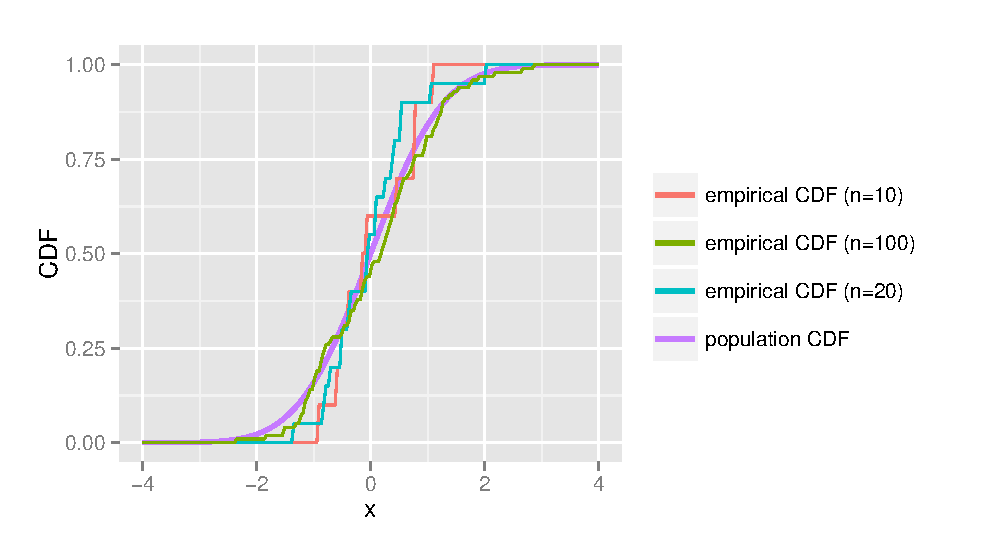
\includegraphics[width=0.9\textwidth]{figures/ch2_ecdf_converge.eps}
\caption{The CDF for the standard Gaussian distribution, accompanied with empirical CDF constructed from sample drawn from the distribution of sizes $ n=10$, $n=20$ and $n=100$. As one can observe from the trend, the gap between the population CDF and the empirical CDF diminishes.}
\label{fig:ch2_ecdf_converge}
\end{center}
\end{figure}

Hence, under convergence, sample moments obtained from a sample with large size are precise estimators for the corresponding population moments, which can be further used to estimate the parameter for the population distribution, which is called \textit{the method of moments}. 

\subsubsection{The method of moments}

Supposing the population distribution  for $ X $ is believe to be $ f(x; \theta_1, \theta_2, \cdots, \theta_p) $, where $ \theta_1, \theta_2, \cdots, \theta_p $ are the parameters to be estimated. From the distribution function, we can calculate the population moments $ \mu_1', \mu_2', \cdots, \mu_p' $, each expressed as a function of $ \theta_1, \theta_2, \cdots, \theta_p $, i.e.
\begin{equation}
\begin{split}
&\mu_1'(\theta_1, \theta_2, \cdots, \theta_p) = \int_{-\infty}^{+\infty} x f(x; \theta_1, \theta_2, \cdots, \theta_p) dx, \\
&\mu_2'(\theta_1, \theta_2, \cdots, \theta_p) = \int_{-\infty}^{+\infty} x^2 f(x; \theta_1, \theta_2, \cdots, \theta_p) dx, \\
&\vdots \\
&\mu_p'(\theta_1, \theta_2, \cdots, \theta_p) = \int_{-\infty}^{+\infty} x^p f(x; \theta_1, \theta_2, \cdots, \theta_p) dx.
\end{split}
\end{equation}
Then we collect the sample moments $ m_1', m_2', \cdots, m_p' $ from data with a large sample size. By equating every population with the corresponding sample moment, we have the equations
\begin{equation}
\begin{split}
&\mu_1'(\theta_1, \theta_2, \cdots, \theta_p) = m_1',\\
&\mu_2'(\theta_1, \theta_2, \cdots, \theta_p) = m_2', \\
&\vdots \\
&\mu_p'(\theta_1, \theta_2, \cdots, \theta_p) = m_p',
\end{split}
\end{equation}
the solution to which provide an estimation for the parameters. And this method of parameter estimation is called the method of moments.

However, the method of moments have been largely superseded by the method of \textit{maximum likelihood estimation} (MLE), which generally gives estimators with a  bigger probability of being close to the parameters to be estimated. Yet, the method of moments can yield the results more quickly and easily by solving the equation, while the MLE may take more time solving an optimization. 

\section{Diverging moments caused by heavy tails}
Previously, we have studied the asymptotic convergence (\textit{asymptotic} in the sense that the sample size $ n \rightarrow \infty $ ) relation between sample and population moments when they exist. Now it is time to move on to exploring the case when population moments diverge. We will see that the divergence of moments is caused by the heavy tails of a distribution, where the probability mass declines to zero with a pace slower than an exponential tail (e.g. the tails in Gaussian). An important member in the heavy-tailed family is the power-law distribution and we will discuss its definition, properties and empirical studies in detail. Meanwhile, it is possible for a heavy-tailed distribution has convergent lower-order moments but divergent higher-order moments. So let us first explore how the \textit{order} of a moment matters. 

% In this case, although we cannot obtain population moments, we can still calculate sample moments from data, as every data point is a finite number. By analyzing the dependence of sample moments on the sample size $ n $, we will see that sample moments \textit{grow with} $ n $. Therefore, we would ask \textit{how fast} does a sample moment grow with sample size, which can be more formally put as the \textit{asymptotic behavior} of a sample moment. Furthermore, is their anyway we can recover (or predict) the asymptotic behavior of a sample moment directly from the population distribution? 
   

\subsection{Moment order}
The theorem below states that for a distribution, if a moment of higher order exists, then every moment of lower order also exists.

\begin{thm}
For a random variable, if the $ n $-th population moment $ \mu_n' $ exists, then  for every $ 0<k \leq n $, $ \mu_k' $ also exists. 
\end{thm}
\begin{proof}
Supposing a random variable $ X $ with PDF $ f(x) $, then
\[ \mu_k' = \int_{-\infty}^{+\infty} x^k f(x) dx \leq \int_{-\infty}^{+\infty} {|x|}^k f(x) dx = \int_{|x|>1} {|x|}^k f(x) dx + \int_{|x|\leq 1} {|x|}^k f(x) dx, \]
where the first term satisfies 
\[ \int_{|x|>1}|x|^k f(x) dx \leq \int_{|x|>1} |x|^n f(x) dx = \int_1^{+\infty} x^n f(x) dx \pm \int_{-\infty}^{-1} x^n f(x) dx, \]
where both terms on RHS are convergent due to the existence of $ \mu_n' $. Meanwhile, it follows that
\[ \int_{|x| \leq 1} |x|^k f(x) dx \leq \int_{-\infty}^{+\infty} f(x) dx = 1. \] Therefore, $ \mu_k' $ is convergent.
\end{proof}

More generally, the existence of $ \mu_n' $ guarantees the convergence of $ \mu_k(c), \ 0<k \leq n $ for any $ c $. Hence, for a distribution, the convergence of moments falls into either category:
\begin{enumerate}
\item There exists a maximum order $ n_c $ for moment to be convergent. Moments with orders less than $ n_c $ are all convergent, while moments with orders higher than $ n_c $ are all divergent.
\item Moments of all orders are convergent ($ n_c=\infty $ ).
\end{enumerate}

The convergence of moment is only a problem when a distribution has a tail (the range of distribution extends to infinity on one side) or has two tails (the range extends to infinity on both sides); distributions with $ x $ bounded to a finite range always have convergent moments. By recalling how an improper integral is defined, we can see that the convergence of a population moment solely depends on the \textit{shape of its tail (or tails)}. For distributions with exponentially bounded tails, $ n_c = \infty $; for heavy-tailed distributions, we can expect $ n_c < \infty $.  

\subsection{Heavy-tailed distribution}
Supposing the CDF for a function is $ F(x) $, then a distribution (not limited to a finite range) is said to have an exponentially bounded \textit{right tail} if there exists some $ \lambda>0 $ such that 
\begin{equation}
\lim_{x \rightarrow +\infty} e^{\lambda x} (1-F(x)) < \infty,
\end{equation}
or an exponentially bounded \textit{left tail} if there exists some $ \lambda >0 $ such that 
\begin{equation}
\lim_{x \rightarrow -\infty} e^{- \lambda x} F(x) < \infty.
\end{equation}
As the definitions above imply, an exponentially bounded tail vanishes to zero as fast as an exponential function with some $ \lambda>0 $ or faster than that. Either left or right, exponentially bounded tails guarantee the existence of moments of all positive orders, i.e. $ n_c = \infty $, which is an immediate result from that $ \lim_{x \rightarrow \infty} e^{-x} x^n = 0 $ holds for any $ n $. 

However, if a tail vanishes to zero slower than $ any $ exponential function with $ \lambda>0 $, we call it a heavy-tail and it causes moments with order higher than some $ n_c $ diverge. For the sake of simplicity, we restrict tails discussed here to be \textit{right tails}, which can be extended to left tails in a similar fashion. 

\begin{defn}
The distribution of a random variable $ X $ with its CDF $ F(x) $ is said to have a heavy tail if 
\begin{equation}
\lim_{x \rightarrow +\infty} e^{\lambda x} (1-F(x)) = \infty \quad \text{for all} \ \lambda > 0.
\end{equation}
\end{defn}
This definition is equivalent to the statement that the moment generating function $ M(t) $ is infinite for any $ t>0 $ \cite{rolski2009stochastic}. 

Some common distributions with heavy-tails are listed as below.\\
Those that are one-tailed include
\begin{itemize}
\item the power-law distribution (also referred to as \textit{Pareto distribution}),
\item the log-normal distribution,
\item the Levy distribution.
\end{itemize}
Those that are double-tailed include
\begin{itemize}
\item the Cauchy distribution,
\item the t-distribution.
\end{itemize}

As a typical example of heavy-tail with both abundant empirical evidence and theoretical studies, we now briefly outline the definition and properties of \textit{power-law distributions}, which are also referred to as \textit{Pareto distributions}. 

\subsubsection{Power-law distribution}
For the sake of simplicity, we assume the random variable here to be continuous. For a random variable $ X $ obeying power-law distribution, its PDF is in the form of
\begin{equation}
f(x) = \frac{\alpha -1}{x_{\min}} (\frac{x}{x_{\min}})^{-\alpha}, 
\end{equation}
where $ x $ is defined on the range $ [x_{\min}, +\infty) $ and $ x_{\min}>0 $ is a cut-off on the minimum value for $ X $. $ \alpha>1  $ is called the \textit{scaling exponent}, its value being bigger than $ 1 $ is required for power-law to be normalizable.

The name \textit{scale exponent} is due to a property of power-law called \textit{scale invariance}. Scaling the variable $ X $ by a positive constant $ c $ only causes a proportionate scaling of the PDF itself, that is 
\begin{equation}
f(cx) = c^{-\alpha} f(x),
\end{equation}
where $ \alpha $ characterizes the power of the homogeneous function. Therefore, two power-laws with the same scaling exponent are equivalent up to a constant factor, with one being a \textit{scaled} version of the other. To simplify the expression for the PDF, one can scale $ X $ by dividing it by $ x_{min} $. Then the resulting random variable $ X' = X/x_{min} $ has the PDF with the same $ \alpha $, i.e.
\begin{equation}
f_{X'}(x) = (\alpha-1) x^{-\alpha}.
\end{equation}

\begin{figure}[!h]
\begin{center}
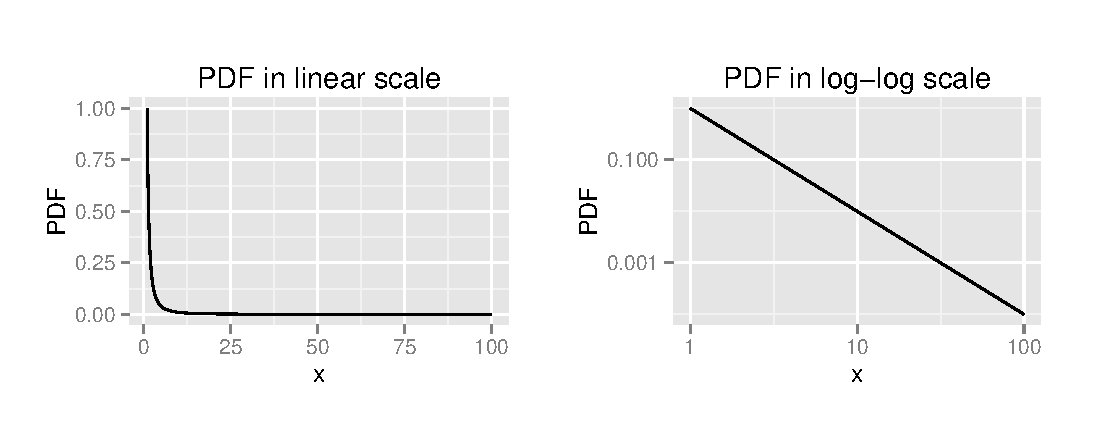
\includegraphics[width=0.9\textwidth]{figures/ch2_powerlaw_pdf.eps}
\caption{The PDF for a power-law with $ x_{\min}=1 $ and $ \alpha=2 $. The figure on the left in plotted in linear-linear scale and the figure on the right is plotted in log-log scale.}
\label{fig:ch2_powerlaw_pdf}
\end{center}
\end{figure}

Fig. \ref{fig:ch2_powerlaw_pdf} shows the PDF for a power-law distribution in two drawing scales. As the tail for power-law is heavier than a exponential one, the length of the power-law tail can be very long (the maximum of $ x $ in data can be very big) compared to the length of the head, where most of the ``probability mass'' is concentrated. Hence, a power-law is often preferred to be drawn in a log-log scale. By taking logarithm on both sides of the PDF, we can see that the logarithm of the PDF is related to the logarithm of the variable in a linear relation, with the slope being just $ -\alpha $, i.e.
\begin{equation}
\log f(x) = -\alpha	\log (x) + \log[(\alpha-1) x_{\min}^{\alpha-1}].
\end{equation}
Meanwhile, to see if a variable follows a power-law from data, it is often handy to plot the probability versus the value in log-log scale and see if is basically a straight line. However, without a following rigorous treatment for parameter estimation and statistical test, a naive graphical method for identifying power-law and estimating the exponent can be misleading \cite{Clauset2009}. 

To observe the heavy tail for power-law more straightforwardly, we can integrate the PDF to arrive at the CDF as 
\begin{equation}
F(x) = 1 - (\frac{x}{x_{\min}})^{1-\alpha}.
\end{equation}
It follows that for any $ \lambda>0 $ we have 
\[ \lim_{x \rightarrow +\infty} e^{\lambda x} (1-F(x)) = \lim_{x \rightarrow +\infty} \frac{e^{\lambda x}}{(x/x_{\min})^{\alpha-1}} =0,\]
thus proving that the tail is indeed heavier than an exponential one. 
The \textit{tail distribution} for power-law is given by
\begin{equation}
P(X>x) = 1-F(x) = (x/x_{\min})^{1-\alpha}, 
\end{equation}
which is also a relation expressed by multiplicative power. This form of characterization is often seen when the power-law is called the \textit{Pareto distribution} and the constant $ \beta=\alpha-1 > 0 $ is called the \textit{Pareto index}.

The scaling exponent $ \alpha $ (or the Pareto index $ \beta=\alpha-1 $) characterizes the \textit{heterogeneity} of a power-law distribution. As drawn in Fig. \ref{fig:ch2_alpha}, when $ \alpha \rightarrow \infty $, the distribution approaches to a Dirac delta function, with all probability mass places on a single point, which corresponds to maximal heterogeneity; when $ \alpha \rightarrow 1 $, loosely speaking, the distribution approaches a ``uniform'', where the probability mass is equally places from $ x_{\min} $ to $ \infty $, which corresponds to maximal homogeneity. 

\begin{figure}[!h]
\begin{center}
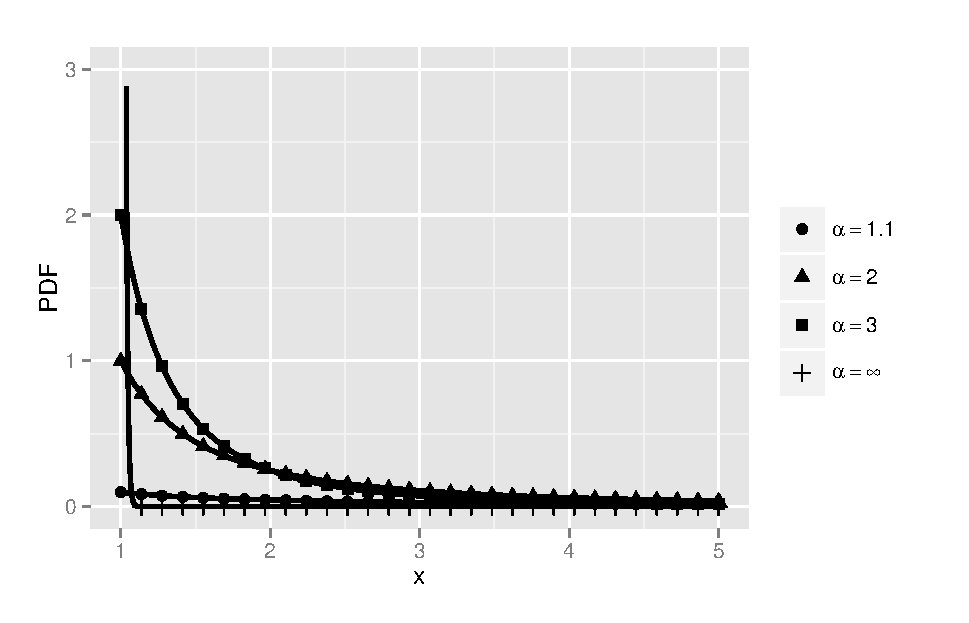
\includegraphics[width=0.9\textwidth]{figures/ch2_alpha.eps}
\caption{PDFs of power-law distributions with $ x_{\min}=1 $ and different values of $ \alpha $. It can be seen that the distribution approaches an uniform distribution when $ \alpha \rightarrow 1 $ (more homogenous), while it approaches a Dirac delta function centered at a single point when $ \alpha \rightarrow \infty $ (more heterogeneous).   }
\label{fig:ch2_alpha}
\end{center}
\end{figure}

Power-law distributions (i.e. Pareto distributions) has been empirically found in an extraordinarily diverse phenomena. Power-law is often connected with the intuition that the data is not centered around a ``typical value'', which is often referred to as \textit{heterogeneity}  For example, the distribution of population of cities and towns is found to follow a power-law: the largest city in US is New York City with more than 8 million residents but the smallest one in US is a small town with about 50 residents only \cite{newman2005power}. The distribution for the population of cities from the US Census in 2000 is drawn by Fig. \ref{fig:ch2_population}, where the straight line in log-log scale matches the form of power-law. Aside from city population, the distributions for the sizes of earthquakes \cite{gutenberg1942earthquake}, solar flares \cite{lu1991avalanches}, the frequency of words in any human language \cite{zipf1949human}, the number of citations received by papers \cite{de1965networks}, the degrees of web pages on the Internet \cite{barabasi1999emergence,faloutsos1999power}, the sales of books and recordings \cite{cox1995concentration}, people's annual incomes \cite{pareto1964cours} have also been found to follow the power-law. 

\begin{figure}[!h]
\begin{center}
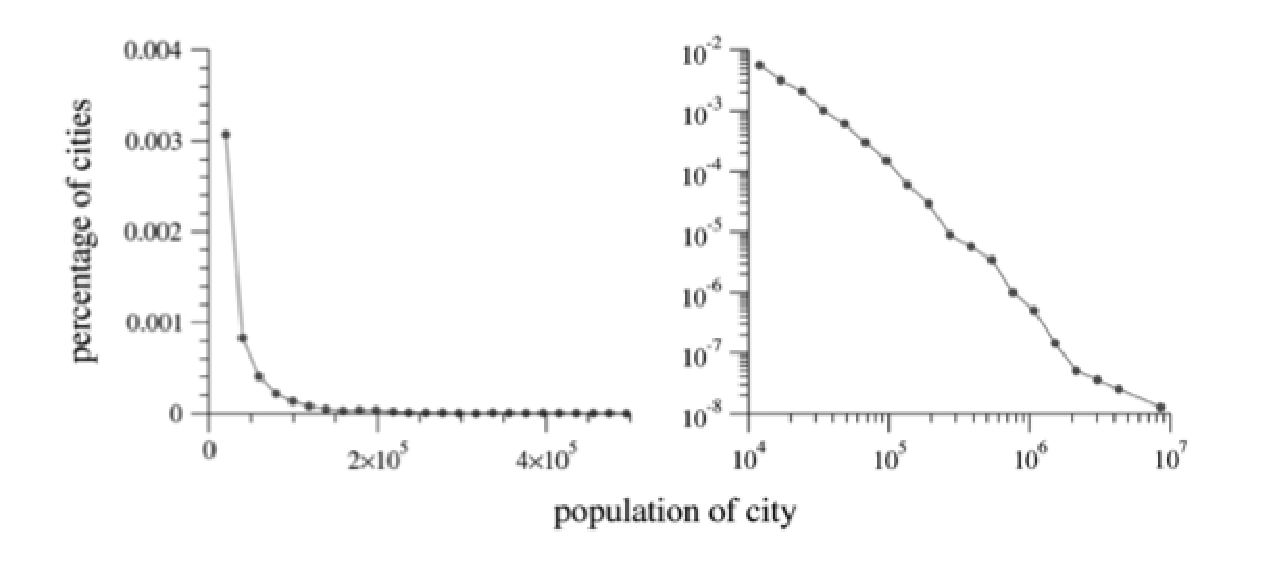
\includegraphics[width=0.9\textwidth]{figures/ch2_population.eps}
\caption{Left: histogram of the populations of all US cities with population of 10000 or more. Right: another histogram of the same data, but plotted on logarithmic scales. The approximate straight-line form of the histogram in the right panel implies that the distribution follows a power law. Data is collected from the 2000 US Census. (figure excerpted from \cite{newman2005power}))}
\label{fig:ch2_population}
\end{center}
\end{figure}

We now take a look at the maximum order $ n_c $  allowed in a power-law for a moment to converge. The $ k $-th raw moment is given by 
\begin{align*}
\mu_{k}' &= \int_{x_{\min}}^{+\infty} \frac{\alpha-1}{x_{\min}} (\frac{x}{x_{\min}})^{-\alpha} x^k dx \\
&= (\alpha-1) x_{\min}^{\alpha-1} \int_{x_{\min}}^{+\infty} x^{k-\alpha} dx = (\alpha-1) x_{\min}^{\alpha-1} \frac{x^{k-(\alpha-1)}}{k-(\alpha-1)} \Bigg|_{x_{\min}}^{+\infty},
\end{align*}
which requires $ \lim_{x \rightarrow +\infty} x^{k-(\alpha-1)} $ to converge. Therefore, we have 
\begin{equation}
k < n_c = \alpha -1
\end{equation}
for a power-law with scaling exponent $ \alpha >1 $. Notably, when $ 2 < \alpha \leq 3 $, the power-law has finite mean but diverging variance; when $ 1 < \alpha \leq 2 $, even the mean diverges.  

\section{Equiprobable partition method}
In this section, we will develop the \textit{equiprobable partition method} (EPM) as a theoretical tool for analyzing the asymptotics of diverging moments. The equiprobable partition method partitions the area under the PDF into slices with equal sizes (i.e. equal probabilities) and use these slices to represent or approximate the samples. We will see that when the moment is convergent, the sample moments given by EPM is consistent with its expectation, i.e. the corresponding population moment (that is to say, EPM is precise in the convergent case); and when the moment is divergent, we can use EPM to reproduce the asymptotic behaviors of the sample moments as the sample size grows. 

Before we go in depth to the method, we shall first explain what happens to sample moments when the corresponding population moments diverge and what we mean by using the word \textit{asymptotics} for sample moments. 

As an illustrative example, we draw ``bags'' of samples from a power-law distribution with $ x_{\min}=1 $ and $ \alpha=2.5 $, where the sample size $ n $ for the ``bag'' is growing. 
\begin{figure}[!h]
\begin{center}
\includegraphics[width=0.7\textwidth]{figures/ch2_moment_grow.eps}
\caption{Sample raw moments $ m_1', m_2', m_3' $ and $ m_4' $  computed from samples drawn from a power-law distributions with $ x_{\min}=1 $ and $ \alpha=2.5 $, plotted against the sample size $ n $ in the log-log scale .  }
\label{fig:ch2_moment_grow}
\end{center}
\end{figure}
Fig. \ref{fig:ch2_moment_grow} draws the sample raw moments $ m_1', m_2', m_3' $ and $ m_4' $ versus size of samples for computing them. Due to $ \alpha=2.5 $, the maximum order for moment to converge is $ n_c = \alpha-1=1.5 $. Therefore, as shown in the figure, only $ m_1' $ converges to its expectation $ \frac{\alpha -1}{\alpha -2}=3 $. Other moments $ m_1' $, $ m_2' $ and $ m_3' $ clearly \textit{grows with the sample size} (although the growth may look unsteady with fluctuations, the general increasing trend is obvious by referring to the exponentially spaced numbers on the y-axis). In other words, instead of converging to a fixed value, these sample moments continue to grow as more data is accumulated. The growth of a divergent sample moment relying on the sample size $ n $ when $ n \rightarrow \infty $ is what we call the \textit{asymptotic behavior} of the sample moment, or its \textit{asymptotics}. With the aid of \textit{equiprobable partition method}, we can approximate a diverging moment in the form of $ n^{\gamma} g(n) $, where $ n^{\gamma} $ characterizes the \textit{leading order} of divergence (thus answering: \textit{how fast is the divergence?} ) and $ g(n) < \infty \ (n \rightarrow \infty ) $ is a function of $ n $ that characterizes the sample moment's ``convergence'' by cutting off the divergence (thus answering: \textit{what is left in the moment other than the leading order?}).

\subsection{Equiprobable partitions}
Similar to the \textit{partition} defined in Riemann integrals (or Riemann-Stieltjes integrals), a \textit{equiprobable partition} is a list of points that cut the range for $ x $ into consecutive intervals. But, as its name suggests, the equiprobable partition is special in that it cuts the $ x $-axis in the way that the area of the PDF above every interval is \textit{the same}, so that a random sample falls into every interval with \textit{equal probability}. We will discuss why we choose such a partition scheme later.

Let us denote a partition that produces $ n $ intervals with $ \mathcal{P}_n $, which is called a \textit{$ n $-separated partition}.  The partition $ \mathcal{P}_n $ for a random variable defined on the interval $ [a,b] $ is defined as below.
\begin{defn}
Let $ X $ be a continuous random variable defined on the interval $ [a, b] \in \mathbb{R} $ with the PDF $ f(x)\ (a \leq x \leq b) $, then its $ n $-separated partition $ \mathcal{P}_n (a,b) $ is defined as 
\begin{equation}
\mathcal{P}_n (a,b) = (\hat{t}_0, \hat{t}_1, \cdots, \hat{t}_n),
\end{equation}
where $ \hat{t}_0 = a $, $ \hat{t}_n=b $ and it satisfies that 
\begin{equation}
\int_{\hat{t}_i}^{\hat{t}_{i+1}} f(x) dx = \frac{1}{n} \quad (i=1,2,\cdots, n-1).
\end{equation}
\end{defn}

It directly follows from the definition that the interval points can be obtained from the CDF $ F(x) $ as
\begin{equation}
F(\hat{t}_i) = \frac{i}{n} \quad (i=0,1,\cdots,n)
\end{equation}
If we assume that the PDF $ f(x) $ is a well-defined function, then its integral $ F(x) $ should be an increasing function, of which the inverse function $ F^{-1}(x) $ must exist. The interval points can thus be uniquely determined by the inverse function of CDF, i.e.
\begin{equation}
\hat{t}_i = F^{-1} (\frac{i}{n}) \quad (i=0,1,\cdots, n).
\end{equation}
Fig. \ref{fig:ch2_partition_schematic} is a schematic illustration of a partition $ \mathcal{P}_n(a,b) $ with $ n=9 $. Clearly, the interval points are not evenly spaces. Instead, the density for interval points is high when $ f(x) $ is large and is low when $ f(x) $ is small, which is consistent with how samples are distributed in regions with different probability densities. 
\begin{figure}[htbp]
\begin{center}
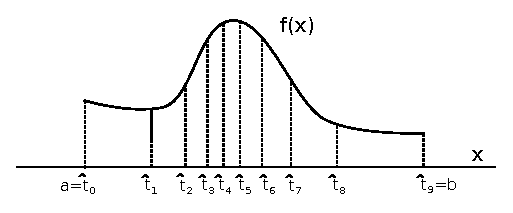
\includegraphics[width=0.9\textwidth]{figures/ch2_partition_schematic.eps}
\caption{A schematic of illustration of $ P_9(a,b) $. Instead, the density for interval points is high when f(x) is large and is low when f(x) is small, which is consistent with how samples are distributed in regions with different probability densities.}
\label{fig:ch2_partition_schematic}
\end{center}
\end{figure}

Hence, we can use the interval points in equiprobable partitions to \textit{approximate sample points}. In the Riemann integral, one point picked in each interval in the partition as the \textit{representative point} for that interval, and the partition is said to be \textit{tagged} by these representative points. How one picks the representative points does not matter as long as the Riemann sum converges when the maximum length of intervals diminishes to zero. Similarly, in our case, to every interval we assign a representative point placed in the interval. As the positioning of this point inside the interval does not matter when $ n \rightarrow \infty $, for convenience, we just pick the left end $ \hat{t}_{i} $ for the interval $ [\hat{t}_i, \hat{t}_{i+1}] $ as the \textit{representative point} .  

Now, we use $ n $ representative points $ \{ \hat{t}_0, \hat{t}_1, \cdots, \hat{t}_{n-1} \}$ derived from an $ n $-separated equiprobable partition to approximate a sample $ \{ x_1, x_2, \cdots, x_n \} $ of size $ n $. That is to say, the set of points $ \{ \hat{t}_0, \hat{t}_1, \cdots, \hat{t}_{n-1} \} $ as a whole is an approximation for the set of samples $ \{x_1, x_2, \cdots, x_n\} $ as a whole, while the ordering among the elements in each does not matter. 

Meanwhile, because we know that $ \hat{t}_0 \leq \hat{t}_1 \leq \cdots \leq \hat{t}_{n-1} $, we first sort the samples and then use $ \hat{t}_{i} $ as an approximation for the $ (i+1) $-th smallest sample. In other words, the determinant points $ (\hat{t}_0, \hat{t}_1, \cdots, \hat{t}_{n-1}) $ can be used to estimate the \textit{order statistics} for a distribution, where both the ordering among $ \{\hat{t}_i\} $  and the ordering among samples after sorting shall be taken into account.

For now, we focus on the first case where ordering does not matter. By using $\{ \hat{t}_0, \hat{t}_1, \cdots, \hat{t}_{n-1} \}$ to approximate the samples $ \{ x_1, x_2, \cdots, x_n \} $, we seek to construct estimators for sample moments. 

\subsection{EPM estimators for sample moments}
Every sample moment taken at point $ c $ is a polynomial function of sample points, i.e.
\begin{equation}
m_{k}(c) = \frac{1}{n} \sum_{i=1}^{n} (x_i-c)^k.
\end{equation}
The EPM (equiprobable partition method) estimator for the sample moment is constructed by simply \textit{replacing the samples $ \{x_1, x_2, \cdots, x_n\} $ with the representative points $ \{ \hat{t}_0, \hat{t}_1, \cdots, \hat{t}_{n-1} \} $}.  

\begin{defn}
Given a random variable $ X $ and a sample of size $ n $ independently drawn from its distribution, the EPM (equiprobable partition method) estimator for the $ k $-th sample moment $ m_k(c) $ is defined to be
\begin{equation}
\hat{m}_k(n;c) = \frac{1}{n} \sum_{i=1}^{n} (\hat{t}_{i-1}-c)^k,
\end{equation}
which is a function of $ n $. The interval points $ \{ \hat{t}_0, \hat{t}_1, \cdots, \hat{t}_{n} \} $ are given by the $ n $-separated equiprobable partition $ \mathcal{P}_n $ for $ X $. 
\end{defn}

We now show that when $ X $ is a random variable defined on a finite interval and its PDF is bounded. Then the EPM moment estimator is \textit{unbiased} when $ n \rightarrow \infty $, that is it coincides with population moment. We will show that, in fact, an EPM moment estimator is in fact the same as the Riemann-Stieltjes integral for the corresponding population moment when $ n $ extends to infinity.

\begin{thm}
Let $ X $ be a random variable defined on the interval $ [a, b] $ with its PDF $ f(x) \  (a \leq x \leq b) $. Supposing $ f(x) $ is bounded, i.e. there exists some $ M $ that it holds that $\forall x \in [a, b]$, $f(x) < M$, we have 
\begin{equation}
\lim_{n \rightarrow \infty} \hat{m}_{k}'(n) = \mu_k',
\end{equation}
where $ \hat{m}_{k}'(n) = \frac{1}{n} \sum_{i=1}^n (\hat{t}_{i-1})^k $ is the EPM estimator for $ k $-th raw moment, $ \mu_k' $ is the $ k $-th population moment. \label{thm:epm_consistent}
\end{thm} 

\begin{proof}
From the definition of $ \mathcal{P}_n(a,b) $, we have
\begin{align*}
\frac{1}{n} &= F(\hat{t}_i) - F(\hat{t}_{i-1}) \quad (i=1,2,\cdots,n) \\
&= f(\hat{t}_{i-1})(\hat{t}_i - \hat{t}_{i-1}) + o(\hat{t}_{i}-\hat{t}_{i-1}).
\end{align*}
For an $ \epsilon>0 $ that is small enough, if $ \hat{t}_i - \hat{t}_{i-1} < \epsilon $, then we have $ o(\hat{t}_{i}-\hat{t}_{i-1}) < \delta (\hat{t}_i - \hat{t}_{i-1}) $ for some $ \delta>0 $. Meanwhile, due to the bound $ f(x)<M $, we have
\[ \frac{1}{n} < (M+\delta)(\hat{t}_{i}-\hat{t}_{i-1}). \]
Therefore, for any small $ \epsilon>0 $, when $ n > \frac{1}{(M+\delta)\epsilon} $, we shall have $ (\hat{t}_i - \hat{t}_{i-1})<\epsilon $. That is, 
\[ \lim_{n \rightarrow \infty} \max_{1 \leq i \leq n} (\hat{t}_i - \hat{t}_{i-1}) = 0, \]
showing that the \textit{mesh} for the partition vanishes to zero when $ n \rightarrow \infty $.  
Meanwhile, the EPM estimator can be rewritten as
\begin{align*}
\lim_{n \rightarrow \infty} \hat{m}_k'(n) &= \lim_{n \rightarrow \infty} \frac{1}{n} \sum_{i=1}^n (\hat{t}_{i-1})^k \\
&= \lim_{n \rightarrow \infty} \sum_{i=1}^n (\hat{t}_{i-1})^k [F(\hat{t}_i) - F(\hat{t}_{i-1})].
\end{align*}
Hence, by the definition of Riemann-Stieltjes integral, we have 
\[ \lim_{n \rightarrow \infty} \hat{m}_{k}'(n) = \int_{a}^b x^k dF(x) = \mu_k'. \]
\end{proof}

By expanding a moment taken about $ c $, we arrive at the following conclusion immediately. 
\begin{lemma}
For a random variable $ X $ with bounded PDF $ f(x) < M \ (a \leq x \leq b) $, we have 
\begin{equation}
\lim_{n \rightarrow \infty}{\hat{m}_k (n)} = \mu_k,
\end{equation}
\begin{equation}
\lim_{n \rightarrow \infty}{\hat{m}_k (n;c)} = \mu_k(c).
\end{equation}
\end{lemma}
That is to say, the EPM estimators for sample central moments or moments taken about any point coincide with population moment, if $ X $ is a random variable with finite range and bounded PDF. To arrive at these conclusions, we have assumed that the PDF is bounded, which applies to most well-defined distributions and only rules out those with \textit{generalized functions} (e.g. PDFs containing Dirac's delta).

\subsection{Asymptotics for diverging moments}
Having proven that EPM estimators are \textit{precise} when moments converge, we now extend the usage of EPM estimators to deriving the asymptotics of diverging sample moments. For convenience, in this section we assume that $ X $ is a random variable \textit{with a heavy tail on the right side}, while right-tailed or double-tailed distributions can be analyzed in a similar fashion. Let $ f(x) \ (a \leq x < +\infty) $ be the PDF for $ X $ and $ f(x)$ is bounded by some $ M $. The equiprobable partition for $ X $ is defined by changing $ \mathcal{P}_n(a,b) $ to $ \mathcal{P}_n(a, +\infty) $, that is
\begin{equation}
\mathcal{P}_n(a, +\infty) = (\hat{t}_0, \hat{t}_1, \cdots, \hat{t}_{n-1}, \hat{t}_n),
\end{equation}
where $ \hat{t}_0=a $ and $ \hat{t}_{n}=+\infty $. The representative points $ \{\hat{t}_0, \hat{t}_1, \cdots, \hat{t}_{n-1}\} $ are given by 
\begin{equation}
F(\hat{t}_i) = \frac{i}{n} \quad (i=0,1,\cdots,n-1),
\end{equation}
where it shall be noted that the probability mass from the maximum representative to infinity is also $ 1/n $. That is to say, the EPM imposes an upper cut-off on approximated samples and the probability of drawing a random sample beyond the cut-off is $ 1/n $, which vanishes to zero when $ n \rightarrow \infty $. 
  
The $ k $-th sample moment $ m_k(c) $ computed from a sample of size $ n $ is approximated by the EPM estimator $ \hat{m}_k(n;c) $, which is constructed by substituting the sample points with representative points from the $ n $-separated equiprobable partition, i.e.
\begin{equation}
\hat{m}_k (n;c) = \frac{1}{n} \sum_{i=1}^n (\hat{t}_{i-1}-c)^k.
\end{equation}

Then, we rewrite $ \hat{m}_k(n) $ ($ c $ is left out for simplicity) into the form of 
\begin{equation}
\hat{m}_k(n) = n^{\gamma} g(n),
\end{equation}
where $ n^\gamma $ is the \textit{leading order} that characterizes the speed of convergence. And $ g(n) $ is a function that satisfies 
\begin{equation}
0 < \lim_{n \rightarrow \infty} |g(n)| < \infty,
\end{equation}
which is the ``convergent term'' for sample moments formed by deducting the effect of divergence from the sample moment.

To showcase the analytical procedure above, we use this machinery to find the asymptotics for the first several diverging moments of the power-law distributions with $ \alpha < 3 $ and compare them to numerical results. 

Here we assume the lower cut-off $ x_{\min}=1 $, and the PDF is given by 
\begin{equation}
f(x) = (\alpha-1) x^{-\alpha},
\end{equation}
and the CDF is given by
\begin{equation}
F(x) = 1 - x^{1-\alpha}.
\end{equation}
We use the CDF to construct the $ n $-separated equiprobable partition $ \mathcal{P}_n(1, +\infty) $. From the relation
\begin{equation}
F(\hat{t}_i) = 1-(\hat{t}_i)^{1-\alpha} = \frac{i}{n} \quad (i=0,1,\cdots, n-1),
\end{equation}
we have the representative point as 
\begin{equation}
\hat{t}_i = (1-\frac{i}{n})^{-c}, 
\end{equation}
where we adopt a shorthand $ c = \frac{1}{\alpha-1} > \frac{1}{2}$. When $ \alpha \leq 3$, the maximum order for convergent moment is $ n_c=\alpha-1 < 2 $, here we present the asymptotics for diverging sample raw moments $ m_k' $ with $ k \geq 2 $.

The EPM estimator for $ m_k' $ is 
\[ \hat{m}_k'(n) = \frac{1}{n} \sum_{i=0}^{n-1} (\hat{t}_i)^k = \frac{1}{n} \sum_{i=0}^{n-1} (1-\frac{i}{n})^{-ck},\]
which can be rewritten as the product of a leading order term and a ``convergent'' term, i.e.
\begin{equation}
\hat{m}_k'(n) = \frac{1}{n} \sum_{i=0}^{n-1} n^{ck} (n-i)^{-ck} = n^{ck-1} \sum_{i=1}^n \frac{1}{i^{ck}}.
\end{equation}
Therefore, the leading order for the $ k $-th diverging raw moment is $ n^{ck-1} \ (ck>1)$, and a higher order $ k $ means a faster divergence with $ n $.  The ``convergent'' term is 
\begin{equation}
g(n) = \sum_{i=1}^n \frac{1}{i^{ck}} \quad (ck>1),
\end{equation}
and its limit is the famous \textit{Riemann zeta function}
\begin{equation}
\lim_{n \rightarrow \infty} g(n) = \zeta(ck).
\end{equation}
Therefore in limit of $ n \rightarrow \infty $, the EPM asymptotics for sample moments are given by
\begin{equation}
\hat{m}_{k}'(n) \approx n^{ck-1} \zeta(ck).
\end{equation}

\begin{figure}[!h]
\begin{center}
\includegraphics[width=0.8\textwidth]{figures/ch2_powerlaw_asymptotics.eps}
\caption{The comparison between numerical sample moments $ \hat{m}_3 $, $ \hat{m}_4 $ $ \hat{m}_5 $ (cross) and their EPM asymptotics (line). The divergence can be effectively characterized by the asymptotics. Sample moments fluctuate around the theoretical line due to randomness.}
\label{fig:ch2_powerlaw_asymptotics}
\end{center}
\end{figure}

In Fig. \ref{fig:ch2_powerlaw_asymptotics}, we compare the sample moments computed from numerical experiments with their asymptotics given by EPM for $ k=2,3,4 $. That the diverging sample moments fluctuate around their asymptotics shows that the equiprobable partition method is valid in two aspects: the leading order is correct, so that the slope matches the speed of divergence with different orders; the remaining ``convergent'' term is correct, so that the intercept match the positioning of points. 

\subsection{EPM estimators for order statistics}
As mentioned earlier, the ordering among representative points given by EPM can also be utilized to construct estimators for order statistics, i.e. the sorted samples. 

\begin{defn}
Given $ X $ as a random variable and supposing $ X_1, X_2, \cdots, X_n $ are $ n $ i.i.d. samples drawn from the distribution, then the \textit{order statistics}   ${X_{(1)}, X_{(2)}, \cdots, X_{(n)}}$ for the samples are defined by sorting the samples in the increasing order. That is $ X_{(1)}, X_{(2)}, \cdots, X_{(n)} $ is a permutation of the samples that satisfies 
\begin{equation}
X_{(1)} \leq X_{(2)} \leq \cdots \leq X_{(n)}.
\end{equation}
\end{defn}

The representative points given by an $ n $-seperated equiprobable partition naturally satisfies 
\begin{equation}
t_0 < t_1 < \cdots < t_{n-1}.
\end{equation}
Therefore, we can use the $ i $-th smallest EPM representative point to estimate the $ i $-th smallest sample, i.e.
\begin{equation}
\hat{X}_{(i)} = t_{i-1} \quad (i=1, 2, \cdots, n).
\end{equation}

For most cases in asymptotic analysis for sample moments, it is \textit{unnecessary} to use the estimators for order statistics, as sample moments are defined to be \textit{permutational invariant}. For example, the variance is the same for samples $ X_1, X_2, X_3 $ and $ X_3, X_2, X_1 $, where the ordering among samples does not matter.

Yet, the EPM estimators for order statistics is useful when addressing the statistics where the ordering among elements is concerned, e.g. those in \textit{time series}. 
In the following Chapter, we will see a scenario that applies EPM estimators to obtaining the bounds of a statistic with regard to all permutations of the time series.

\subsection{Why equiprobable}
We have introduced the equiprobable partition method and used it as an estimation for samples and order statistics. The reader may be curious about the reason behind the principle of cutting the probability mass into slices of \textit{equal probabilities}, which plays a central role in the magic of EPM. Now, instead of a rigorous argument towards its mathematical necessity, we just briefly outline the intuitive \textit{rationale} behind this principle. 

\begin{enumerate}
\item A equiprobable partition ensures that the \textit{mesh} of the partition vanishes to zero as the number of partitions increases. 

This has been proven by Theorem \ref{thm:epm_consistent} and is important to guarantee that the estimator is unbiased when the moment converges. Of course, it is possible to propose other schemes of partitioning with the same mesh-vanishing property. 

\item The equiprobable partition reaches maximum entropy. 

Let us view a partition as a way to \textit{discretize} a continuous distribution. Then, for a $ n $-separated partition, there are $ n $ outcomes with one outcome corresponding to one interval. Let $ p_i \ (i=1,2, \cdots, n)$ be the probability of a random sample falls into the $ i $-th interval, then the entropy for this discrete distribution would be 
\begin{equation}
H = -\sum_{i=1}^{n} p_i \log(p_i).
\end{equation}
And the configuration $ p_1 = p_2 = \cdots = p_n = \frac{1}{n} $, as used in EPM, is the only one that maximizes the entropy. The principle of maximum entropy has been applied in statistics, information theory and statistical mechanics and reader may refer to the discussions in \cite{jaynes1957information,jaynes1957information2,jaynes1988relation} by Jaynes.

\item It is easy to determine interval ends in the equiprobable partition. 

For most well-defined distributions, the interval ends and therefore the representative points can be easily and uniquely determined with $ F^{-1}(x) $. This is important in practical applications. 

\end{enumerate}






